\documentclass[11pt,a4paper]{article}
\usepackage[utf8]{inputenc}
\usepackage[T1]{fontenc}
\usepackage[polish]{babel}
\usepackage{lmodern}
\usepackage[margin=2.2cm]{geometry}
\usepackage{graphicx,booktabs,float,amsmath,hyperref,caption,enumitem}
\graphicspath{{../results/figures/}}
\captionsetup{font=small}
\setlist{nosep}

\title{Deep Learning w Biometrii --- spotkania \#1,2,3\\[2pt]
\large Weryfikacja biometryczna cross-day na podstawie ruchu w VR}
\author{Wojciech Gosiewski \and Mateusz Prokopiuk \and Jakub Jaromski \and Michał Niechciałkowski}
\date{\today}

\begin{document}
\maketitle

\begin{abstract}
Na korpusie \textit{VR-Biometric-Authentication} (41 uczestników, systemy Quest, Vive, Cosmos) przeprowadzono
eksperyment weryfikacji biometrycznej \textit{cross-day}: modele uczono na rzutach z pierwszego dnia, a testowano
na rzutach z drugiego. Porównano trzy architektury (Multi-Input Branch CNN, GRU, Transformer), wykonano ablację
modalności (pozycje / kąty obrotu / oba) i urządzeń (prawy kontroler / hełm / lewy kontroler), a reprezentacje porównano
metodą RSA. Najlepszy wynik osiągnął dwukierunkowy GRU na pełnym zbiorze cech:
Rank-1 = 93,7\% (Quest), 95,9\% (Vive), 90,3\% (Cosmos), EER 1,1--3,9\%.
Najwięcej informacji biometrycznej niesie prawy (rzucający) kontroler. Geometria embeddingów zależy przede
wszystkim od danych wejściowych, a w drugiej kolejności od architektury.
\end{abstract}

\section{Cel i zakres}
Zrealizowano wszystkie punkty polecenia: (1) EDA korpusu, (2) weryfikację cross-day (dzień 1 $\rightarrow$ dzień 2),
(3) trzy klasyfikatory, (4) ocenę metryką Rank-1 z podobieństwem cosinusowym, (5) eksperyment ablacyjny modalności,
(6) analizę reprezentacji RSA. Embeddingi zapisywano w plikach \texttt{train\_embedding.npz} i \texttt{test\_embedding.npz}
dla każdej konfiguracji i każdego seeda.

\section{Eksploracyjna analiza danych (EDA)}
\subsection{Struktura korpusu}
Wykorzystano wstępnie przetworzone pliki \texttt{DatasetsNumpy/\{Quest,Vive,Cosmos\}\{1,2\}.npy}. Każdy plik to jedna sesja
o kształcie $(41, 10, 135, 21)$: 41 uczestników $\times$ 10 kolejnych rzutów $\times$ 135 klatek
(3\,s od chwycenia piłki, $\approx$45\,Hz) $\times$ 21 cech. Cechy to, dla prawego kontrolera, hełmu i lewego kontrolera,
pozycja $(x,y,z)$ w metrach, kąty Eulera $(x,y,z)$ w radianach oraz nacisk spustu. Łącznie mamy
$6 \times 410 = 2460$ sekwencji. Sesje 1 i 2 każdego systemu traktujemy jako „dzień 1” i „dzień 2”.

\begin{itemize}
\item \textbf{Rozkład klas jest idealnie zbalansowany}: każdy uczestnik ma dokładnie 10 rzutów w każdej z 6 sesji (60 nagrań, rys.~\ref{fig:classes}).
  W problemie 41-klasowym nie trzeba więc ważyć klas ani stosować oversamplingu.
\item \textbf{Jakość}: brak wartości NaN i brakujących sekwencji. Spust hełmu jest stale zerowy, zgodnie z dokumentacją.
  Spust lewego kontrolera w sesji Quest1 jest w całości zerowy, a w pozostałych sesjach prawie nieużywany.
  Plik \texttt{Prior*.npy} zawiera tylko 16 niezerowych uczestników z wcześniejszego badania i pominięto go.
\item \textbf{Kąty Eulera} mają nieciągłość $\pm\pi$ (rys.~\ref{fig:euler}). Kąt $y$ hełmu skupia się blisko $-\pi/2$,
  czyli w obszarze blokady przegubu (\textit{gimbal lock}). Dlatego każdy kąt kodujemy parą $(\sin\theta, \cos\theta)$.
\item \textbf{Przebieg rzutu} (rys.~\ref{fig:traj}): sekwencja ma wyraźną strukturę (uniesienie, zamach, wyrzut, opuszczenie ręki).
  Moment puszczenia spustu przypada średnio na 1,5\,s (Quest), 1,2\,s (Vive) i 1,4\,s (Cosmos) (rys.~\ref{fig:trigger}).
  Trajektorie jednej osoby są powtarzalne między dniami, ale niektórzy uczestnicy (np.\ nr~7) mają duży rozrzut czasowy
  i wykonują kilka zamachów.
\item \textbf{Różnice między systemami} (rys.~\ref{fig:possys}): układy współrzędnych systemów różnią się
  (np.\ średnia wysokość hełmu: Quest 2,08\,m, Vive 2,16\,m, Cosmos 1,96\,m). Każdy system modelujemy więc osobno,
  a standaryzację wyliczamy ze zbioru treningowego danego systemu.
\end{itemize}

\begin{figure}[H]\centering
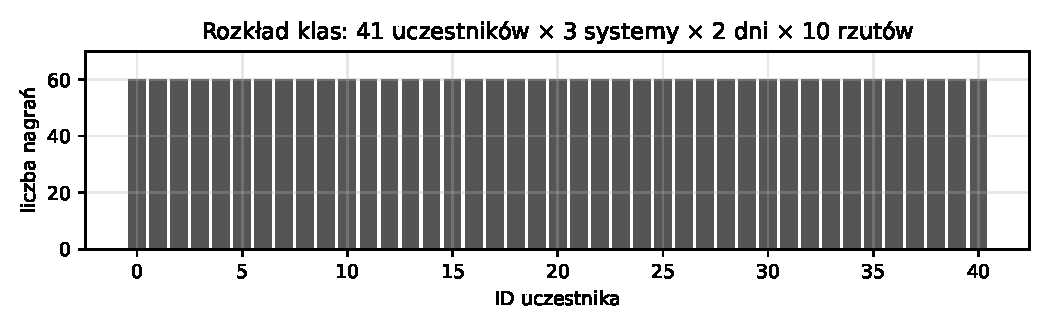
\includegraphics[width=0.75\linewidth]{eda_class_dist.pdf}
\caption{Rozkład klas: 60 nagrań na uczestnika (3 systemy $\times$ 2 dni $\times$ 10 rzutów).}\label{fig:classes}
\end{figure}

\begin{figure}[H]\centering
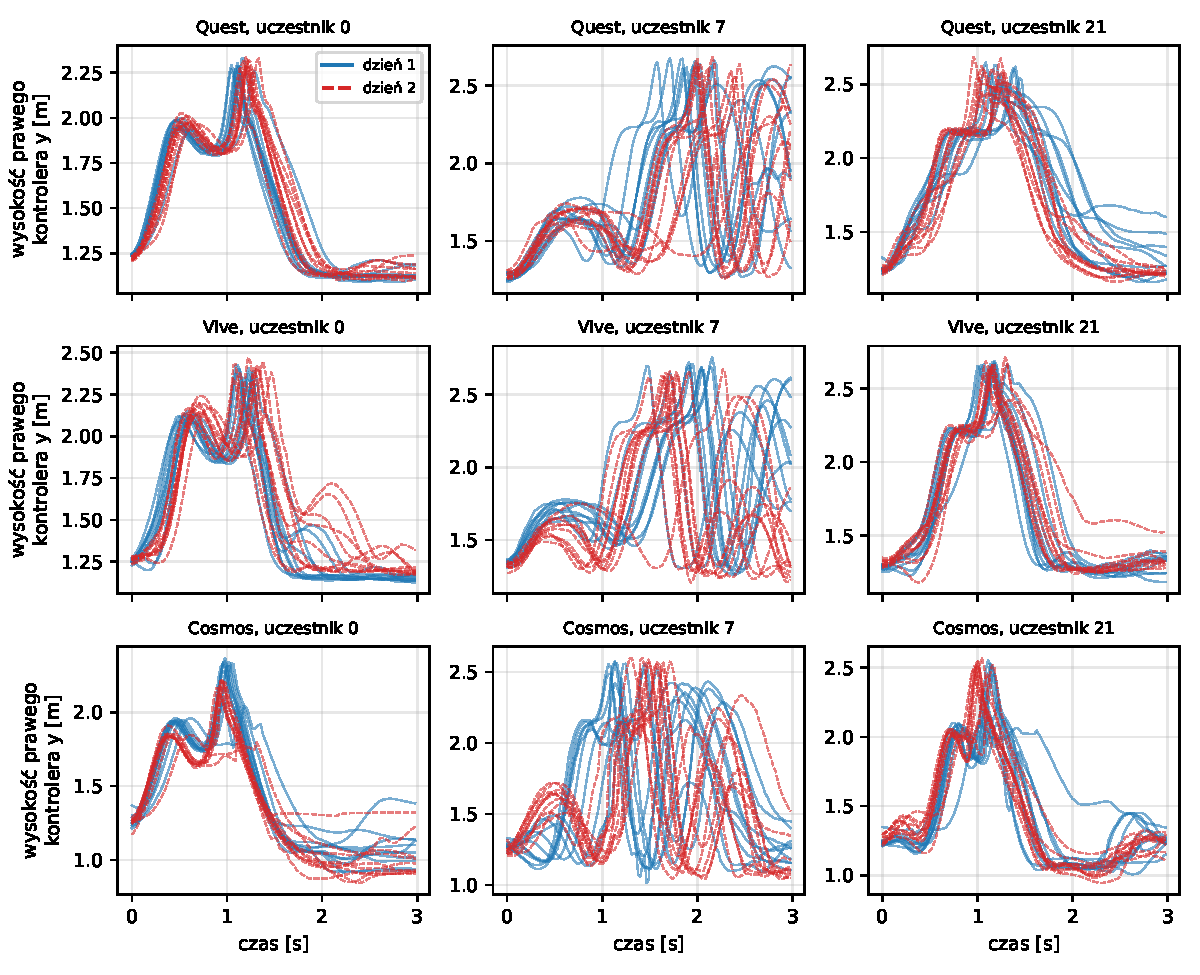
\includegraphics[width=0.85\linewidth]{eda_trajectories.pdf}
\caption{Wysokość prawego kontrolera w czasie dla trzech uczestników: dzień 1 (niebieski) i dzień 2 (czerwony).}\label{fig:traj}
\end{figure}

\begin{figure}[H]\centering
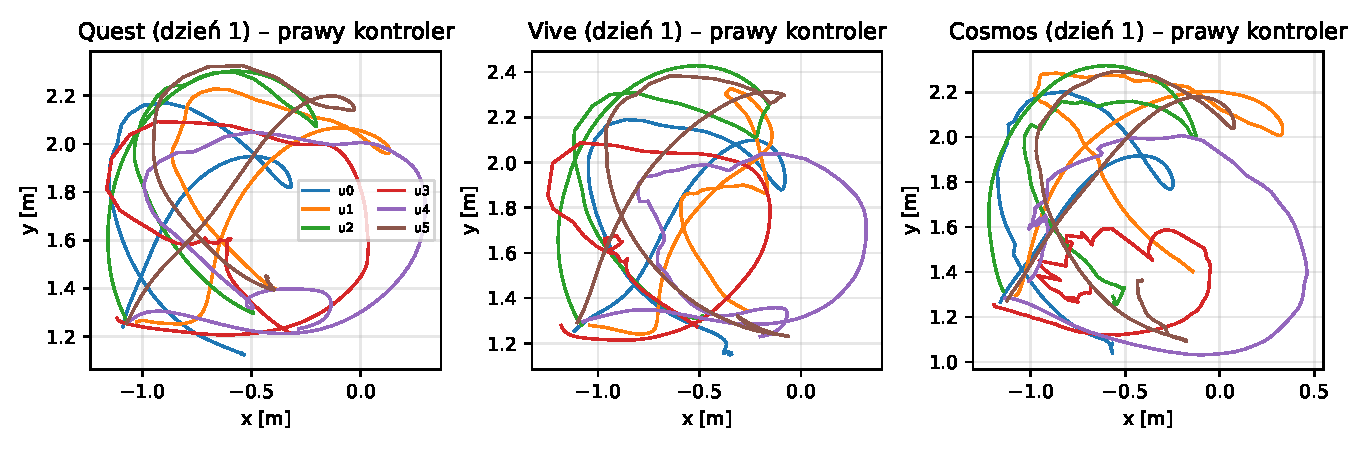
\includegraphics[width=0.9\linewidth]{eda_xy_paths.pdf}
\caption{Średnia ścieżka prawego kontrolera w płaszczyźnie $x$--$y$ (widok z boku) dla 6 uczestników.}
\end{figure}

\begin{figure}[H]\centering
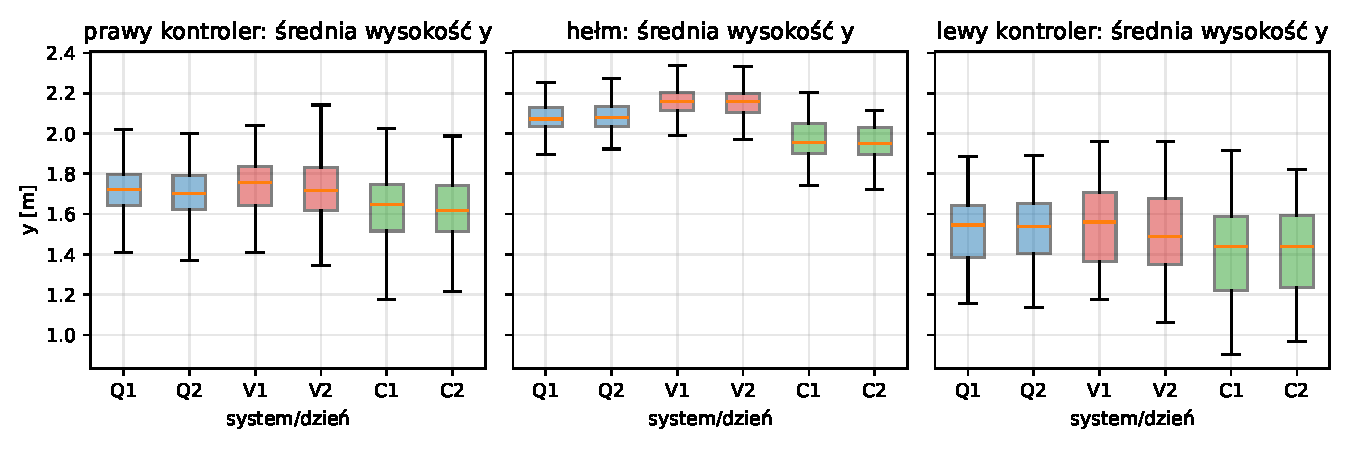
\includegraphics[width=0.9\linewidth]{eda_pos_by_system.pdf}
\caption{Średnia wysokość urządzeń w zależności od systemu (Q/V/C) i dnia (1/2).}\label{fig:possys}
\end{figure}

\begin{figure}[H]\centering
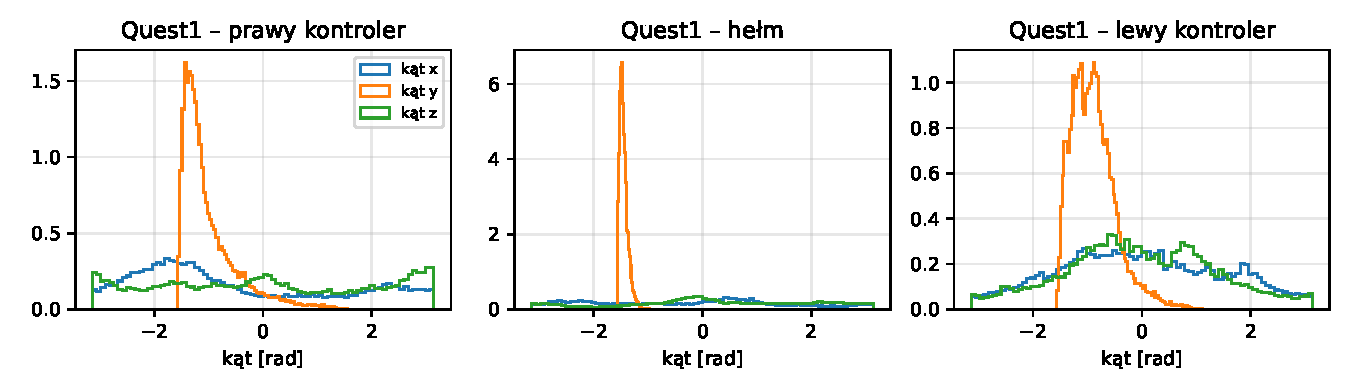
\includegraphics[width=0.9\linewidth]{eda_euler_hist.pdf}
\caption{Rozkłady kątów Eulera (Quest1): przeskoki na granicy $\pm\pi$ uzasadniają kodowanie sin/cos.}\label{fig:euler}
\end{figure}

\begin{figure}[H]\centering
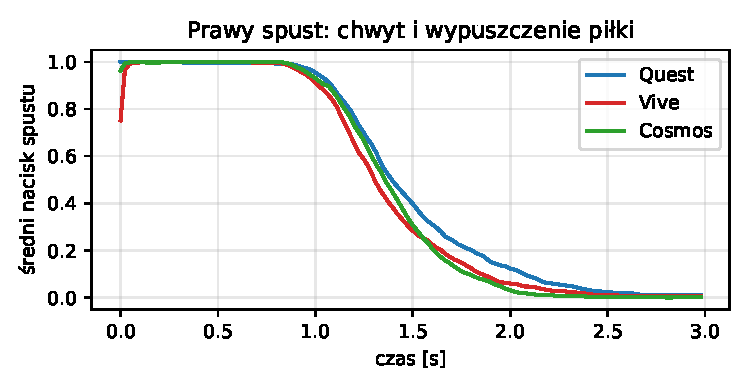
\includegraphics[width=0.5\linewidth]{eda_trigger.pdf}
\caption{Średni nacisk prawego spustu: chwyt piłki (t=0) i jej wypuszczenie.}\label{fig:trigger}
\end{figure}

\subsection{Separowalność i stabilność międzydniowa}
Dla cech uśrednionych w czasie policzono współczynnik Fishera $F = \sigma^2_{\text{między}}/\sigma^2_{\text{wewnątrz}}$
(rys.~\ref{fig:fisher}). Zdecydowanie najbardziej dyskryminująca jest \textbf{wysokość hełmu} ($F\approx14$--15 we wszystkich systemach),
która odpowiada wzrostowi uczestnika, czyli miękkiej cesze biometrycznej. Kolejna jest wysokość lewego kontrolera ($F$=5,7--10).
Dryf międzydniowy (rys.~\ref{fig:drift}) jest wyraźny: średnia pozycja urządzenia tej samej osoby przesuwa się między dniami
o 8--15\,cm, przy 19--35\,cm między różnymi osobami. Identyfikacja wyłącznie po średniej pozycji jednego urządzenia
daje Rank-1 tylko 22--37\%, więc kluczowa jest dynamika ruchu.

\begin{figure}[H]\centering
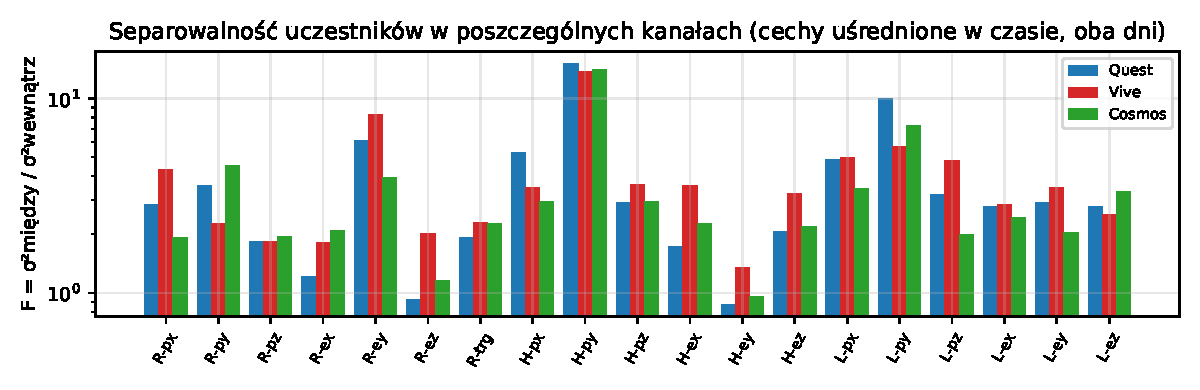
\includegraphics[width=0.9\linewidth]{eda_fisher.pdf}
\caption{Współczynnik Fishera dla kanałów (R/H/L = prawy/hełm/lewy; p = pozycja, e = kąt Eulera, trg = spust).}\label{fig:fisher}
\end{figure}

\begin{figure}[H]\centering
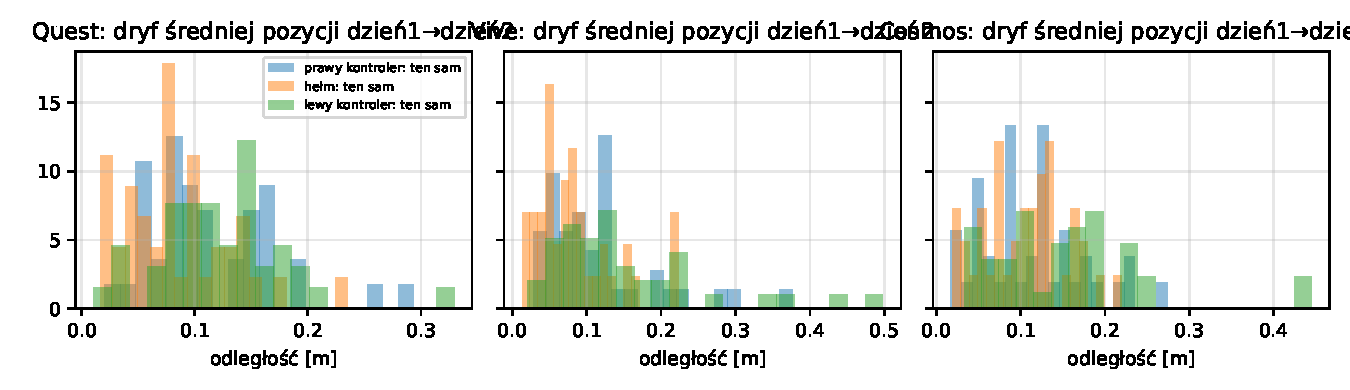
\includegraphics[width=0.9\linewidth]{eda_drift.pdf}
\caption{Przesunięcie średniej pozycji urządzeń tej samej osoby między dniem 1 a dniem 2.}\label{fig:drift}
\end{figure}

\begin{figure}[H]\centering
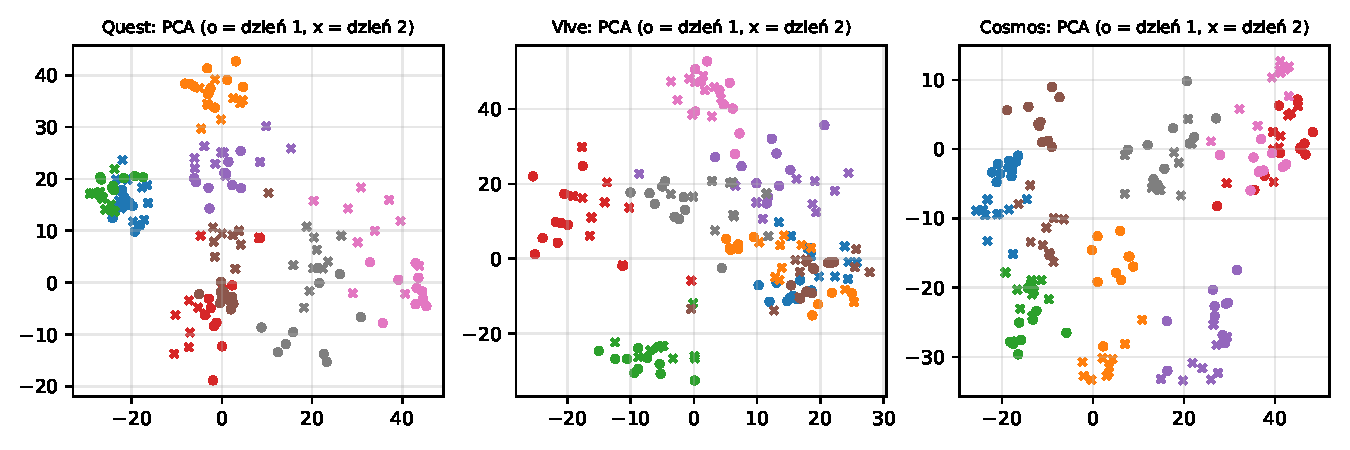
\includegraphics[width=0.9\linewidth]{eda_pca.pdf}
\caption{PCA standaryzowanych, spłaszczonych sekwencji (8 uczestników). Rzuty jednej osoby z obu dni tworzą zwarte skupiska.}\label{fig:pca}
\end{figure}

Projekcja PCA (rys.~\ref{fig:pca}) pokazuje, że już surowe dane są w dużej mierze separowalne.
Jako punkt odniesienia przyjęto więc \textbf{baseline bez uczenia}: podobieństwo cosinusowe między spłaszczonymi,
standaryzowanymi sekwencjami. Uzyskuje on Rank-1 = 85--92\% dla pełnego zestawu cech (tab.~\ref{tab:abl_mod}).

\section{Metodyka}
\subsection{Protokół cross-day i przetwarzanie danych}
Dla każdego systemu osobno: \textbf{zbiór treningowy = sesja 1} (410 sekwencji), \textbf{zbiór testowy = sesja 2} (410 sekwencji),
ci sami 41 uczestnicy (zamknięty zbiór tożsamości). Cechy standaryzowano (z-score per kanał) statystykami
liczonymi \textbf{tylko na zbiorze treningowym}. Dane z dnia 2 nie były wykorzystywane do doboru hiperparametrów ani do
wczesnego zatrzymania: trenowano przez stałą liczbę epok.

Zestawy cech (każde urządzenie: 3 kanały pozycji, 6 kanałów sin/cos kątów; spust pominięto, bo nie należy do żadnej z badanych modalności):
\texttt{pos} (9 kanałów), \texttt{rot} (18), \texttt{all} (27) oraz dodatkowo pojedyncze urządzenia \texttt{right}, \texttt{head}, \texttt{left} (po 9 kanałów, poz.+rot.).

\subsection{Wybór klasyfikatorów}
Wybrano trzy modele z różnych rodzin architektur, żeby porównanie RSA dotyczyło istotnie różnych
uprzedzeń indukcyjnych (konwolucja, rekurencja, atencja):
\begin{itemize}
\item \textbf{Multi-Input Branch CNN (MIB-CNN)}: osobna gałąź Conv1D dla każdego urządzenia
  (3 bloki Conv--BN--ReLU--MaxPool, jądra 7/5/3, 64/64/128 filtrów, global average pooling), fuzja przez konkatenację.
  Struktura odpowiada naturze danych (3 niezależne sensory) i dobrze wychwytuje lokalne wzorce ruchu.
  Ok. 204\,tys.\ parametrów (wariant \texttt{all}).
\item \textbf{GRU}: dwuwarstwowy, dwukierunkowy GRU (96 jednostek), pooling średni i maksymalny po czasie.
  Modeluje zależności czasowe całej sekwencji przy niewielkiej liczbie danych. Ok. 294\,tys.\ parametrów.
\item \textbf{Transformer}: tokenizacja oknami 5 klatek (27 tokenów, $d=64$), uczony embedding pozycji,
  3 warstwy enkodera pre-LN (4 głowice), średnia po tokenach. Ok. 174\,tys.\ parametrów.
\end{itemize}
Wszystkie modele kończą się wspólną głowicą: \texttt{Linear(128)--BN--ReLU--Dropout(0.3)} (\textbf{embedding 128-D}),
a następnie \texttt{Linear(41)} (klasyfikator).

\subsection{Trenowanie}
Funkcja straty: entropia krzyżowa z wygładzaniem etykiet 0,1. Optymalizator AdamW (lr $10^{-3}$, weight decay $10^{-2}$),
harmonogram OneCycle, 150 epok, batch 32, przycinanie gradientu do normy 1. Augmentacja: losowe przesunięcie w czasie
($\pm$10 klatek), skalowanie amplitudy kanałów ($\pm$10\%) i szum gaussowski ($\sigma$=0,05).
Każdą konfigurację trenowano z 3 seedami (0, 1, 2), co daje 3 systemy $\times$ 3 modele $\times$ 6 zestawów cech $\times$ 3 seedy
= \textbf{162 przebiegi}. Jeden przebieg trwał 12--31\,s na GPU RTX 3050 Laptop (PyTorch 2.11).
Krzywe uczenia pokazano na rys.~\ref{fig:curves}.

\begin{figure}[H]\centering
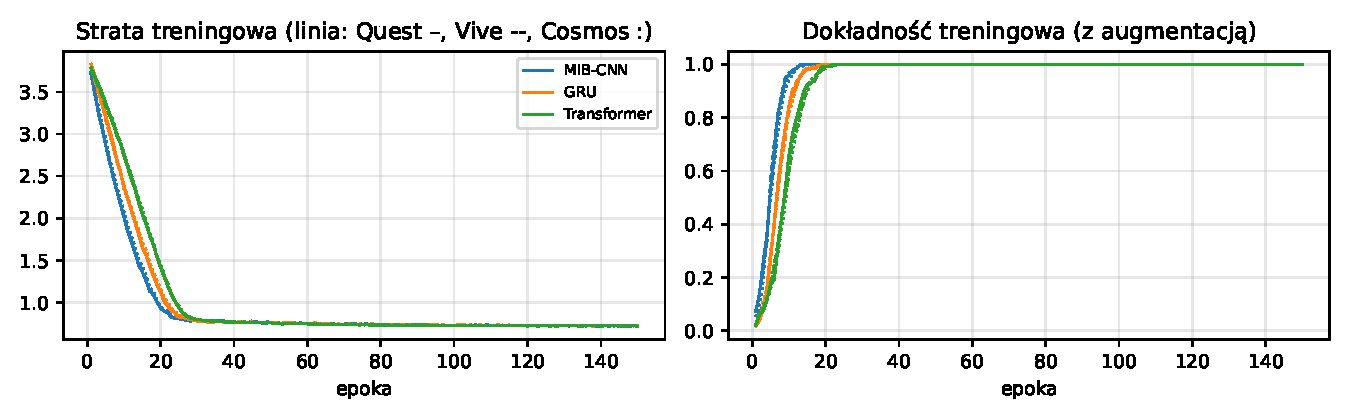
\includegraphics[width=0.85\linewidth]{training_curves.pdf}
\caption{Krzywe uczenia (seed 0, zestaw \texttt{all}).}\label{fig:curves}
\end{figure}

\subsection{Ewaluacja}
Po treningu odcinamy klasyfikator i używamy L2-znormalizowanego embeddingu 128-D:
\begin{itemize}
\item \textbf{Rank-1 (NN)}, metryka główna: dla każdej próby z dnia 2 szukamy najbardziej podobnej (cosinus) próbki galerii z dnia 1.
  Trafienie liczymy, gdy należy ona do tej samej osoby.
\item \textbf{Rank-1 / Rank-5 (szablon)}: galeria to 41 szablonów (średnie embeddingów osoby z dnia 1). Z nich liczymy też krzywą CMC.
\item \textbf{EER}: weryfikacja 1:1, czyli podobieństwo cosinusowe próby do szablonu deklarowanej tożsamości
  (410 par genuine, 16\,400 par impostor).
\end{itemize}

\subsection{Representational Similarity Analysis}
Dla każdej konfiguracji budujemy RDM $D_{ij} = 1-\cos(e_i, e_j)$ na 410 próbach testowych (dzień 2).
Podobieństwo dwóch reprezentacji to korelacja Spearmana górnych trójkątów ich RDM, uśredniona po 3 seedach.
Dodatkowo wyznaczono:
(a) zgodność z idealnym RDM tożsamości, mierzoną jako AUC $P(D_{\text{różne osoby}} > D_{\text{ta sama osoba}})$
(korelacja Spearmana z binarnym RDM nasyca się przy ok. 0,25 z powodu nierównowagi par, więc użyto znormalizowanej wersji);
(b) stabilność międzydniową, czyli Spearmana między RDM centroidów osób ($41\times41$) z dnia 1 i dnia 2;
(c) zgodność między systemami VR (RDM centroidów osób w Quest vs.\ Vive vs.\ Cosmos);
(d) powtarzalność, czyli RSA między seedami tej samej konfiguracji.

\section{Badane scenariusze}
\begin{table}[H]\centering\small
\caption{Scenariusze eksperymentalne.}
\begin{tabular}{p{3.2cm}p{6.8cm}p{5.6cm}}\toprule
Scenariusz & Konfiguracje & Cel \\\midrule
Cross-day & trening sesja 1, test sesja 2; osobno Quest, Vive, Cosmos & stabilność biometrii w czasie \\
Porównanie modeli & MIB-CNN, GRU, Transformer & wybór architektury \\
Ablacja modalności & \texttt{pos}, \texttt{rot}, \texttt{all} & wkład pozycji vs.\ orientacji \\
Ablacja urządzeń & \texttt{right}, \texttt{head}, \texttt{left} & które urządzenie niesie najwięcej informacji \\
Baseline & cosinus na surowych cechach & czy głębokie uczenie coś wnosi \\
RSA & wszystkie powyższe embeddingi & porównanie reprezentacji \\\bottomrule
\end{tabular}
\end{table}

\section{Wyniki}
\subsection{Porównanie klasyfikatorów (pełny zestaw cech)}
\begin{table}[H]\centering\small
\caption{Pełny zestaw modalności (poz.+rot.): porównanie wariantów metryki i kosztu trenowania (średnia z 3 seedów).}\label{tab:full}
\resizebox{\linewidth}{!}{\begin{tabular}{llcccccr}
\toprule
System & Model & Rank-1 NN & Rank-1 szablon & Rank-5 szablon & Acc. softmax & $\bar{s}_{gen}$ / $\bar{s}_{imp}$ & Czas [s] \\
\midrule
Quest & MIB-CNN & 91.8 & 91.8 & 97.8 & 92.3 & 0.83 / 0.34 & 21 \\
 & GRU & 93.7 & 93.7 & 97.6 & 93.9 & 0.83 / 0.33 & 13 \\
 & Transformer & 88.3 & 88.2 & 96.3 & 88.3 & 0.85 / 0.33 & 25 \\
\midrule
Vive & MIB-CNN & 93.7 & 94.1 & 99.5 & 94.1 & 0.84 / 0.33 & 22 \\
 & GRU & 95.9 & 96.0 & 99.9 & 96.7 & 0.85 / 0.33 & 13 \\
 & Transformer & 91.1 & 90.9 & 98.4 & 91.0 & 0.86 / 0.33 & 26 \\
\midrule
Cosmos & MIB-CNN & 88.8 & 88.9 & 97.3 & 89.1 & 0.81 / 0.34 & 20 \\
 & GRU & 90.3 & 90.1 & 96.7 & 90.3 & 0.82 / 0.33 & 12 \\
 & Transformer & 83.1 & 83.4 & 92.4 & 83.0 & 0.82 / 0.33 & 24 \\
\bottomrule
\end{tabular}}
\end{table}

GRU jest najlepszy we wszystkich systemach (średnio 93,3\% Rank-1), przed MIB-CNN (91,4\%) i Transformerem (87,5\%).
Rank-1 liczony względem najbliższej próbki i względem szablonu daje niemal identyczne wartości, a Rank-5 wynosi 92--100\%,
więc błędy to głównie pomyłki z kilkoma podobnymi osobami. Transformer na Vive i Cosmos wypada nieco gorzej niż baseline
bez uczenia (tab.~\ref{tab:abl_mod}). Przy 410 sekwencjach treningowych architektura oparta na atencji jest mocno
niedotrenowana danymi. Na ten problem wskazuje też jej najniższa powtarzalność między seedami (sekcja~\ref{sec:rsa}).
Rozkłady podobieństw genuine/impostor (rys.~\ref{fig:scores}) są dobrze rozdzielone, a nakładanie dotyczy tylko kilku osób.

\begin{figure}[H]\centering
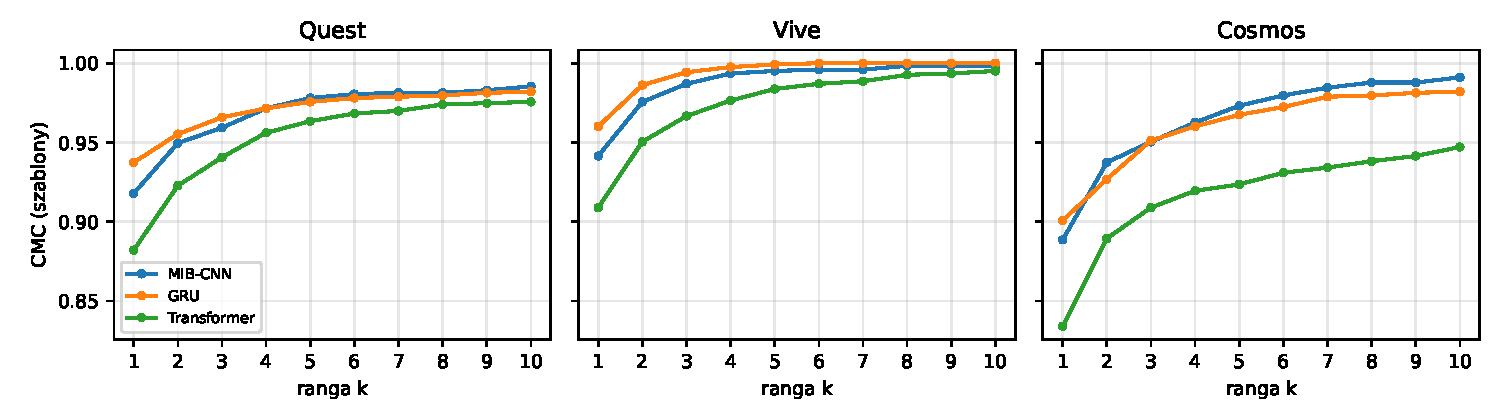
\includegraphics[width=0.9\linewidth]{cmc.pdf}
\caption{Krzywe CMC (szablony, zestaw \texttt{all}, średnia z 3 seedów).}
\end{figure}

\begin{figure}[H]\centering
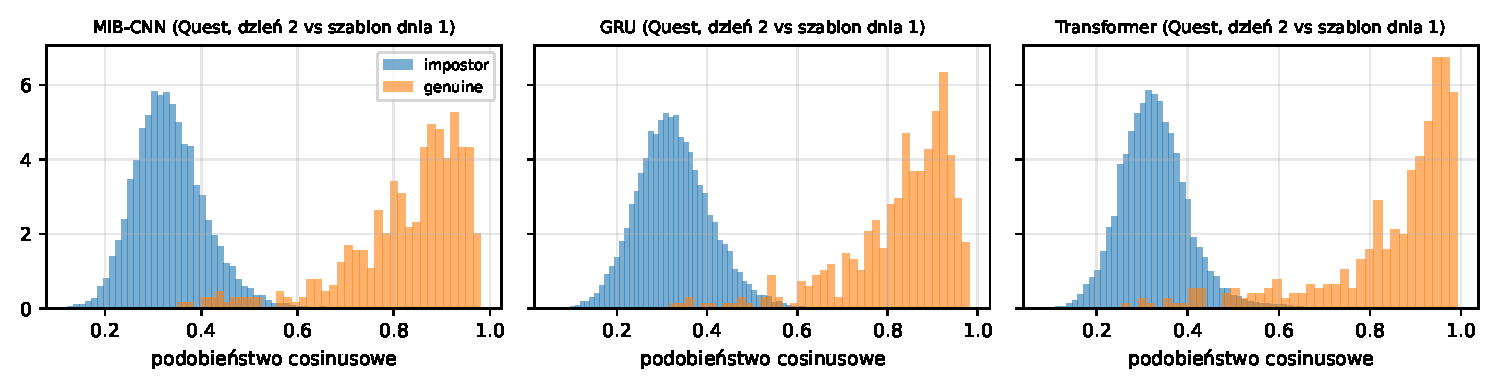
\includegraphics[width=0.9\linewidth]{score_hist.pdf}
\caption{Rozkłady podobieństwa cosinusowego genuine/impostor (Quest, \texttt{all}).}\label{fig:scores}
\end{figure}

\subsection{Ablacja modalności}
\begin{table}[H]\centering\small
\caption{Eksperyment ablacyjny (modalności), weryfikacja cross-day: trening dzień 1, test dzień 2. Średnia $\pm$ odch. std. z 3 seedów. Pogrubiono najlepszy model w danej kolumnie.}\label{tab:abl_mod}
\begin{tabular}{llcccccc}
\toprule
 & & \multicolumn{3}{c}{Rank-1 [\%] (NN, cosinus)} & \multicolumn{3}{c}{EER [\%]} \\
\cmidrule(lr){3-5}\cmidrule(lr){6-8}
Cechy & Model & Quest & Vive & Cosmos & Quest & Vive & Cosmos \\
\midrule
pozycje & MIB-CNN & 88.0$\pm$0.4 & 87.1$\pm$0.9 & 82.8$\pm$1.5 & 4.0$\pm$0.3 & 4.0$\pm$0.5 & 4.2$\pm$0.6 \\
 & GRU & \textbf{92.1$\pm$1.2} & \textbf{90.6$\pm$1.5} & \textbf{88.9$\pm$1.9} & \textbf{2.6$\pm$0.4} & \textbf{2.1$\pm$0.3} & \textbf{3.7$\pm$0.3} \\
 & Transformer & 84.0$\pm$0.9 & 82.1$\pm$1.7 & 82.5$\pm$1.8 & 6.0$\pm$0.3 & 5.6$\pm$0.4 & 6.2$\pm$1.2 \\
 & \textit{surowe cechy} & 81.7 & 86.6 & 82.4 & 11.0 & 10.3 & 10.5 \\
\midrule
rotacje & MIB-CNN & \textbf{88.0$\pm$1.2} & 87.4$\pm$1.2 & \textbf{86.7$\pm$0.9} & \textbf{4.2$\pm$0.1} & \textbf{3.2$\pm$0.5} & \textbf{5.1$\pm$0.8} \\
 & GRU & 87.1$\pm$1.1 & \textbf{88.5$\pm$0.7} & 84.6$\pm$1.5 & 4.4$\pm$1.0 & 3.9$\pm$0.0 & 5.6$\pm$0.4 \\
 & Transformer & 77.5$\pm$2.0 & 77.4$\pm$1.4 & 73.3$\pm$0.6 & 7.7$\pm$1.2 & 7.9$\pm$0.2 & 10.8$\pm$0.2 \\
 & \textit{surowe cechy} & 78.3 & 83.2 & 75.1 & 9.9 & 10.0 & 12.0 \\
\midrule
poz.+rot. & MIB-CNN & 91.8$\pm$1.6 & 93.7$\pm$0.6 & 88.8$\pm$0.7 & 2.8$\pm$0.5 & 1.8$\pm$0.2 & \textbf{3.5$\pm$0.5} \\
 & GRU & \textbf{93.7$\pm$1.4} & \textbf{95.9$\pm$1.3} & \textbf{90.3$\pm$0.1} & \textbf{2.3$\pm$0.4} & \textbf{1.1$\pm$0.3} & 3.9$\pm$0.7 \\
 & Transformer & 88.3$\pm$0.5 & 91.1$\pm$0.5 & 83.1$\pm$2.2 & 3.6$\pm$0.2 & 2.9$\pm$0.2 & 6.8$\pm$0.4 \\
 & \textit{surowe cechy} & 86.8 & 92.0 & 84.9 & 7.6 & 6.3 & 7.5 \\
\bottomrule
\end{tabular}
\end{table}
\begin{figure}[H]\centering
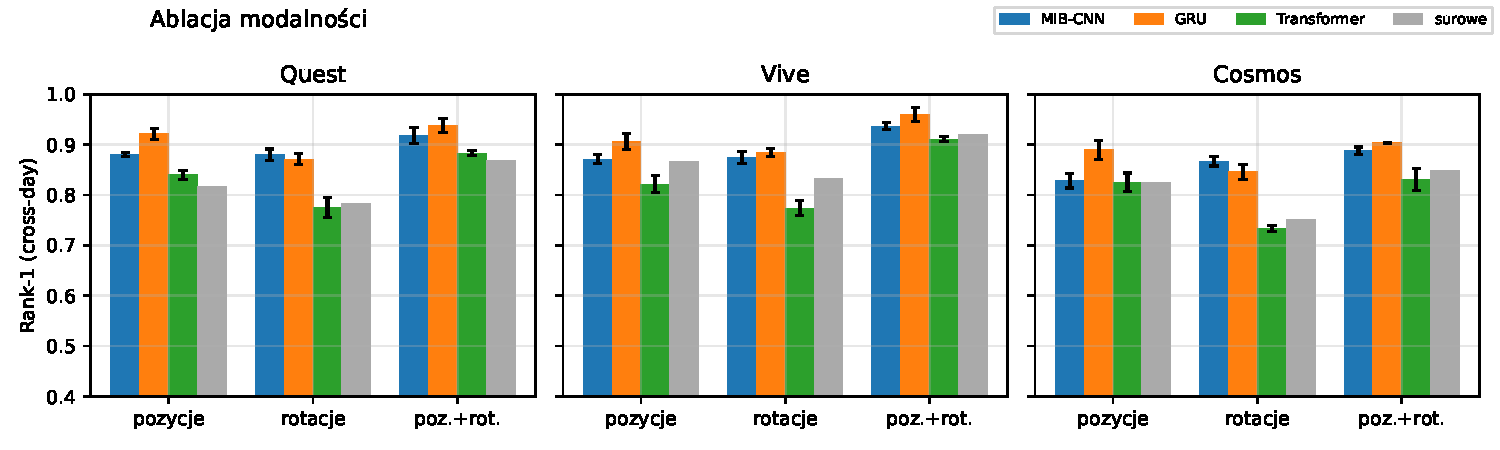
\includegraphics[width=0.95\linewidth]{ablation_modality.pdf}
\caption{Rank-1 cross-day w ablacji modalności (słupki błędu: odch. std. z 3 seedów).}\label{fig:ablmod}
\end{figure}

\begin{itemize}
\item \textbf{Połączenie modalności zawsze pomaga}: średnio +4,3 pp względem samych pozycji i +7,4 pp względem samych rotacji.
  EER spada nawet do 1,1\% (GRU, Vive).
\item Same \textbf{pozycje} są nieco bardziej informatywne niż same \textbf{rotacje} (średnio 86,5\% vs.\ 83,4\%).
  Zawierają bowiem cechy antropometryczne (wzrost, długość ramion), co potwierdza analiza Fishera.
  Wyjątkiem jest MIB-CNN, który lepiej wykorzystuje rotacje (87,3\%) niż pozycje (86,0\%).
\item Transformer wyraźnie najsłabiej radzi sobie z rotacjami (76,1\%), czyli z największą liczbą kanałów (18) przy tak małym zbiorze.
\end{itemize}

\subsection{Ablacja urządzeń}
\begin{table}[H]\centering\small
\caption{Dodatkowa ablacja urządzeń (pozycje + rotacje pojedynczego urządzenia), cross-day, 3 seedy.}\label{tab:abl_dev}
\begin{tabular}{llcccccc}
\toprule
 & & \multicolumn{3}{c}{Rank-1 [\%] (NN, cosinus)} & \multicolumn{3}{c}{EER [\%]} \\
\cmidrule(lr){3-5}\cmidrule(lr){6-8}
Cechy & Model & Quest & Vive & Cosmos & Quest & Vive & Cosmos \\
\midrule
prawy kontr. & MIB-CNN & 90.0$\pm$0.5 & 93.5$\pm$0.4 & 87.9$\pm$1.5 & \textbf{2.5$\pm$0.4} & 1.9$\pm$0.2 & 3.7$\pm$0.4 \\
 & GRU & \textbf{91.9$\pm$1.8} & \textbf{93.7$\pm$0.8} & \textbf{88.0$\pm$1.5} & 3.0$\pm$0.6 & \textbf{1.5$\pm$0.2} & \textbf{3.3$\pm$0.4} \\
 & Transformer & 80.2$\pm$0.7 & 85.5$\pm$1.6 & 81.1$\pm$0.4 & 5.4$\pm$0.2 & 3.4$\pm$0.5 & 5.4$\pm$0.5 \\
 & \textit{surowe cechy} & 71.5 & 78.8 & 74.4 & 14.4 & 11.2 & 13.6 \\
\midrule
hełm & MIB-CNN & 71.8$\pm$0.5 & 76.7$\pm$1.2 & 54.5$\pm$1.4 & 10.0$\pm$1.8 & 4.1$\pm$0.3 & 13.1$\pm$0.5 \\
 & GRU & \textbf{77.5$\pm$1.4} & \textbf{83.8$\pm$1.0} & \textbf{64.2$\pm$2.9} & \textbf{7.7$\pm$0.8} & \textbf{3.3$\pm$0.6} & \textbf{9.3$\pm$1.5} \\
 & Transformer & 72.5$\pm$0.6 & 72.6$\pm$1.5 & 54.6$\pm$0.5 & 9.4$\pm$1.5 & 6.2$\pm$0.5 & 12.9$\pm$1.7 \\
 & \textit{surowe cechy} & 69.5 & 76.3 & 60.0 & 12.7 & 8.8 & 14.1 \\
\midrule
lewy kontr. & MIB-CNN & 68.5$\pm$1.6 & 65.6$\pm$0.2 & 63.2$\pm$0.2 & 10.2$\pm$0.1 & 14.3$\pm$0.8 & 11.3$\pm$0.3 \\
 & GRU & \textbf{74.1$\pm$1.6} & \textbf{67.6$\pm$1.3} & \textbf{69.3$\pm$1.7} & \textbf{7.4$\pm$0.3} & \textbf{13.5$\pm$0.7} & \textbf{10.3$\pm$1.0} \\
 & Transformer & 67.6$\pm$3.1 & 63.9$\pm$1.5 & 66.3$\pm$0.5 & 12.4$\pm$1.5 & 14.2$\pm$0.5 & 13.6$\pm$1.0 \\
 & \textit{surowe cechy} & 69.5 & 66.6 & 62.7 & 13.2 & 16.7 & 15.2 \\
\bottomrule
\end{tabular}
\end{table}
\begin{figure}[H]\centering
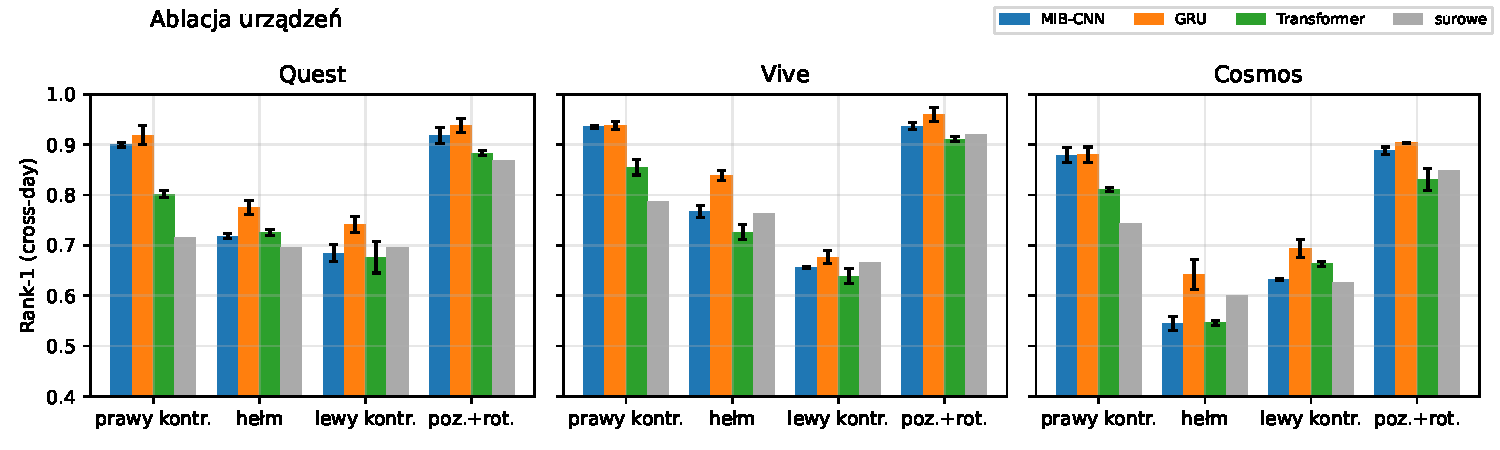
\includegraphics[width=0.95\linewidth]{ablation_devices.pdf}
\caption{Rank-1 cross-day dla pojedynczych urządzeń w porównaniu z kompletem.}\label{fig:abldev}
\end{figure}

\textbf{Prawy kontroler} (ręka rzucająca) niesie zdecydowanie najwięcej informacji. Sam daje średnio 88,0\% Rank-1,
tylko 2,7 pp mniej niż komplet urządzeń, a dla MIB-CNN na Vive praktycznie tyle samo (93,5\% vs.\ 93,7\%).
Hełm (średnio 69,8\%) i lewy kontroler (67,4\%) są znacznie słabsze. Hełm jest szczególnie słaby w Cosmos (57,8\%),
a najlepszy w Vive (77,7\%). Ma przy tym najwyższy współczynnik Fishera dla statycznej wysokości,
więc niesie głównie informację statyczną (wzrost), a mało dynamicznej.

\subsection{Analiza błędów}
\begin{figure}[H]\centering
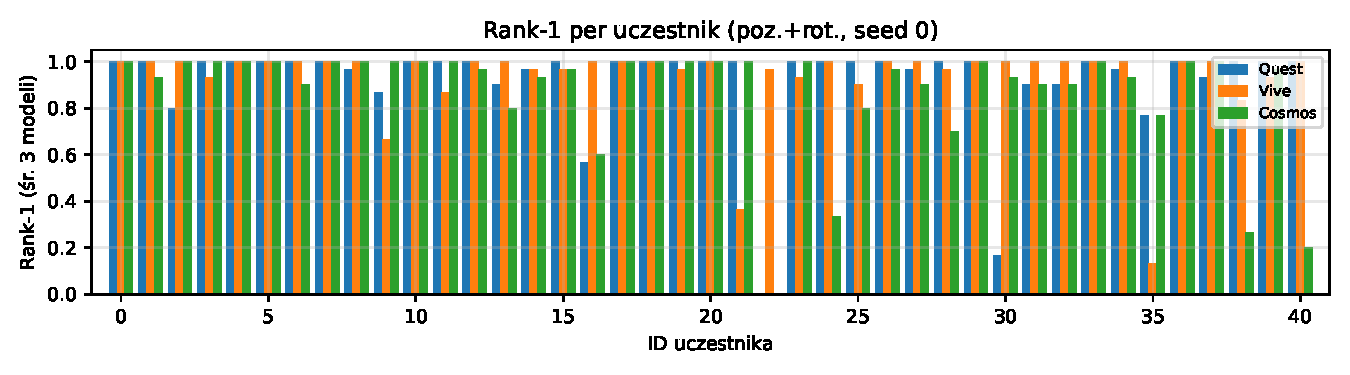
\includegraphics[width=0.9\linewidth]{per_user.pdf}
\caption{Rank-1 w podziale na uczestników (średnia 3 modeli, \texttt{all}, seed 0).}\label{fig:peruser}
\end{figure}
Błędy są silnie skoncentrowane (rys.~\ref{fig:peruser}). Uczestnik 22 w Quest i Cosmos ma Rank-1 = 0, a uczestnik 35 w Vive 13\%.
Przy tym samym uczestniku w innym systemie wynik bywa bliski 100\%. Nie jest to więc błąd etykiet, tylko zmiana sposobu
wykonania rzutu między sesjami (np.\ dla uczestnika 22 w Quest średnia wysokość hełmu zmieniła się o 6\,cm).
Ilustruje to główne wyzwanie biometrii behawioralnej, czyli zmienność wewnątrzosobniczą w czasie.

\begin{figure}[H]\centering
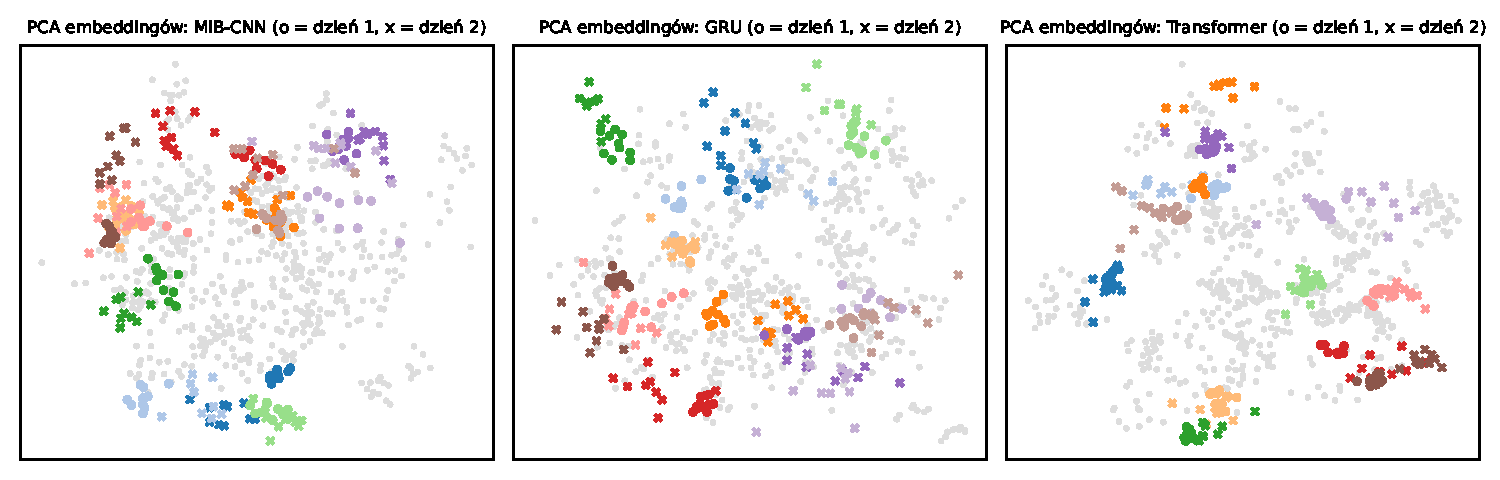
\includegraphics[width=0.9\linewidth]{emb_pca.pdf}
\caption{PCA embeddingów (Quest, \texttt{all}): 12 uczestników w kolorach, reszta na szaro.}
\end{figure}

\section{Analiza reprezentacji (RSA)}\label{sec:rsa}
\begin{figure}[H]\centering
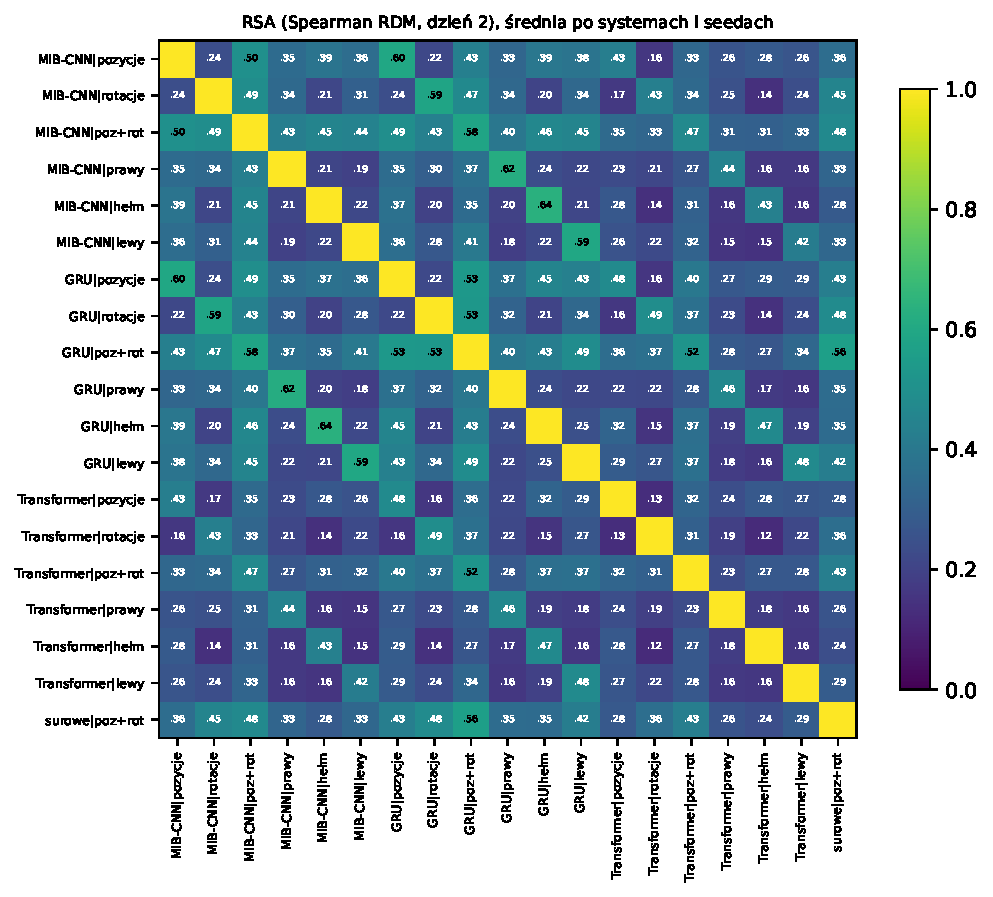
\includegraphics[width=0.8\linewidth]{rsa_configs.pdf}
\caption{Macierz RSA (korelacja Spearmana RDM) między wszystkimi konfiguracjami, średnia po systemach i 3 seedach.}\label{fig:rsa}
\end{figure}

\begin{figure}[H]\centering
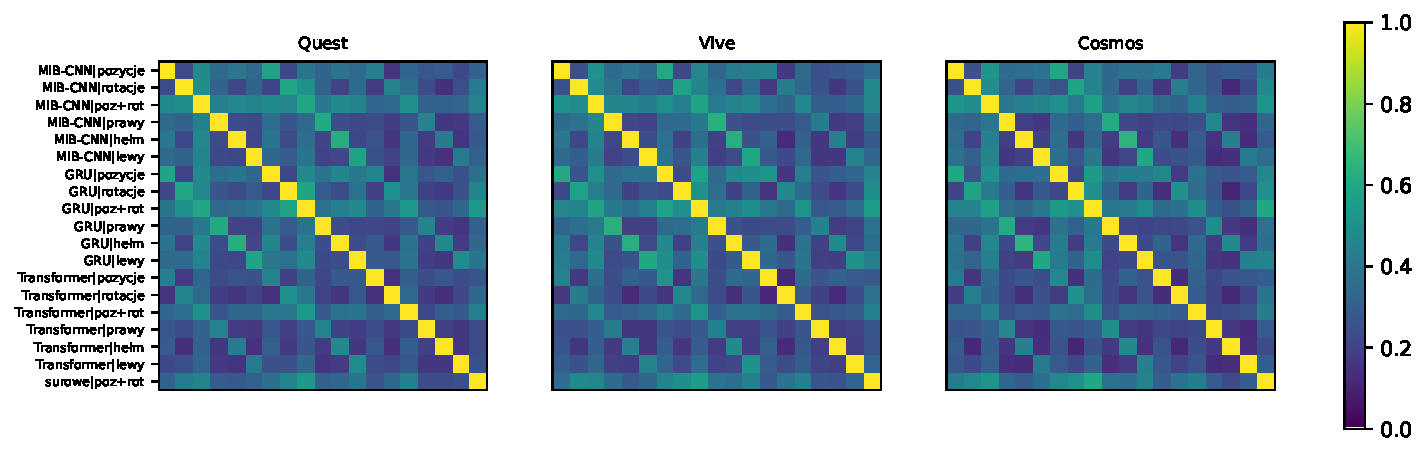
\includegraphics[width=\linewidth]{rsa_configs_per_system.pdf}
\caption{Macierze RSA osobno dla systemów (kolejność wierszy i kolumn jak na rys.~\ref{fig:rsa}); struktura jest spójna między systemami.}
\end{figure}

\begin{figure}[H]\centering
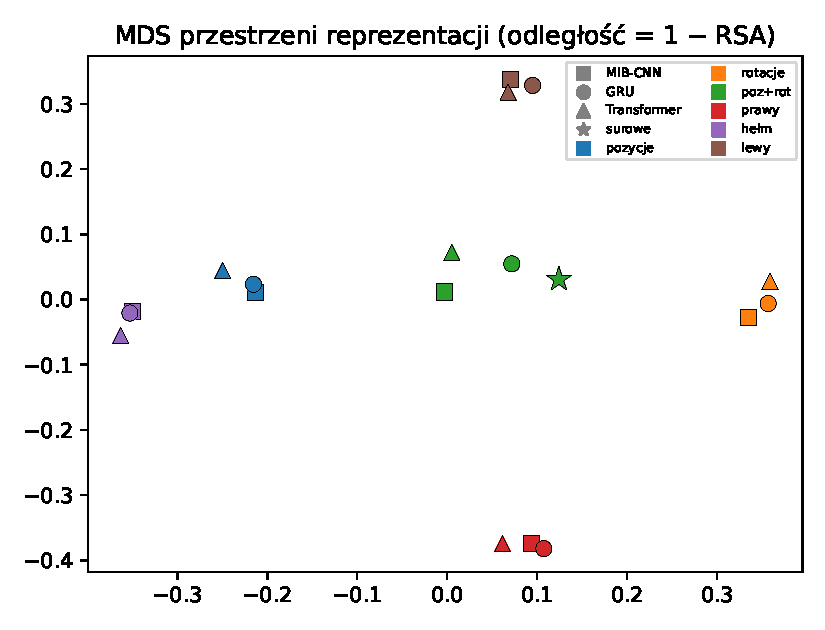
\includegraphics[width=0.6\linewidth]{rsa_mds.pdf}
\caption{MDS konfiguracji w przestrzeni $1-\text{RSA}$ (uśrednione po systemach). Kształt oznacza model, kolor zestaw cech.}\label{fig:mds}
\end{figure}

\begin{itemize}
\item \textbf{Reprezentacja zależy przede wszystkim od wejścia, a nie od architektury.} Na mapie MDS (rys.~\ref{fig:mds})
  konfiguracje grupują się według zestawu cech: trzy modele na tych samych danych leżą obok siebie.
  RSA dla tego samego wejścia i różnych modeli wynosi 0,42--0,64 (np.\ MIB-CNN vs.\ GRU: pozycje 0,60, rotacje 0,59, hełm 0,64).
  Dla tego samego modelu i rozłącznych wejść (pozycje vs.\ rotacje, różne urządzenia) jest to tylko 0,15--0,24
  (np.\ MIB-CNN pozycje vs.\ rotacje: 0,24).
  Pozycje i rotacje oraz poszczególne urządzenia niosą więc \emph{komplementarną} informację o tożsamości,
  co tłumaczy zysk z ich łączenia.
\item Reprezentacje \texttt{all} leżą w centrum mapy MDS, między zestawami cząstkowymi, i są najbardziej podobne do baseline'u
  na surowych cechach (RSA 0,43--0,56). Modele zachowują więc ogólną strukturę danych, a jednocześnie silniej ją porządkują względem tożsamości.
\item \textbf{Zgodność z tożsamością}: AUC rozróżnienia par ta sama/inna osoba na dniu 2 wynosi 0,9987 (MIB-CNN i GRU, \texttt{all}),
  0,9976 (Transformer) i 0,9865 (surowe cechy). Najniższe wartości mają lewy kontroler i hełm (0,984--0,995).
  Ranking jest zgodny z Rank-1.
\item \textbf{Stabilność międzydniowa} (RDM centroidów osób, dzień 1 vs.\ dzień 2) jest najwyższa dla prawego kontrolera
  (0,54--0,59) i najniższa dla lewego (0,33--0,40). Surowe cechy mają wyższą stabilność (0,57--0,64) niż embeddingi (0,33--0,59):
  sieci uczone na klasyfikację rozpychają osoby równomiernie i porzucają część „naturalnych” podobieństw między nimi.
\item \textbf{Zgodność między systemami VR} (te same osoby, różny sprzęt) jest niska: 0,22--0,33 dla embeddingów (najwyższa dla GRU)
  i 0,28--0,41 dla surowych cech. Relacje podobieństwa między osobami tylko częściowo przenoszą się między urządzeniami,
  co ma znaczenie dla scenariuszy cross-device.
\item \textbf{Powtarzalność między seedami}: GRU 0,75, MIB-CNN 0,71, Transformer 0,45. Transformer uczy się za każdym razem
  innej geometrii, co wraz z niższą skutecznością wskazuje na niedobór danych dla tej architektury.
\end{itemize}

\begin{figure}[H]\centering
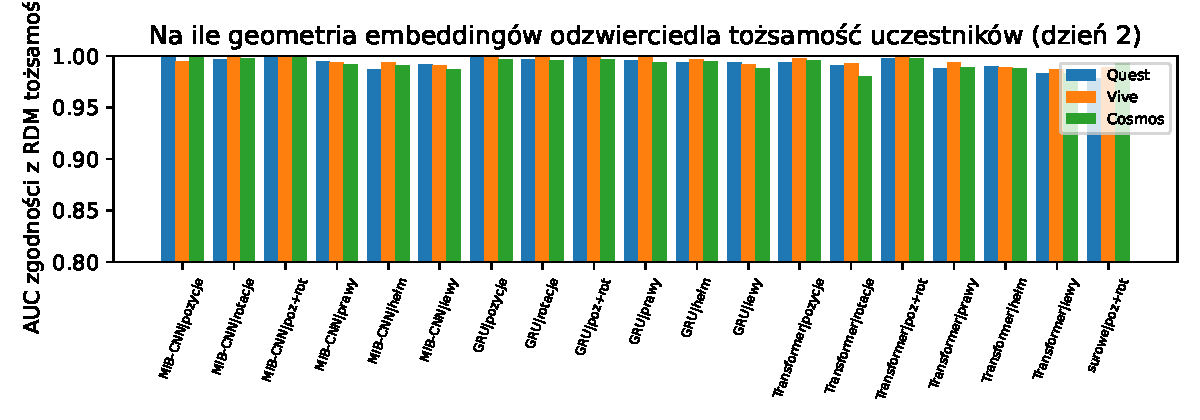
\includegraphics[width=0.9\linewidth]{rsa_identity.pdf}
\caption{AUC zgodności RDM z idealnym RDM tożsamości (dzień 2).}
\end{figure}
\begin{figure}[H]\centering
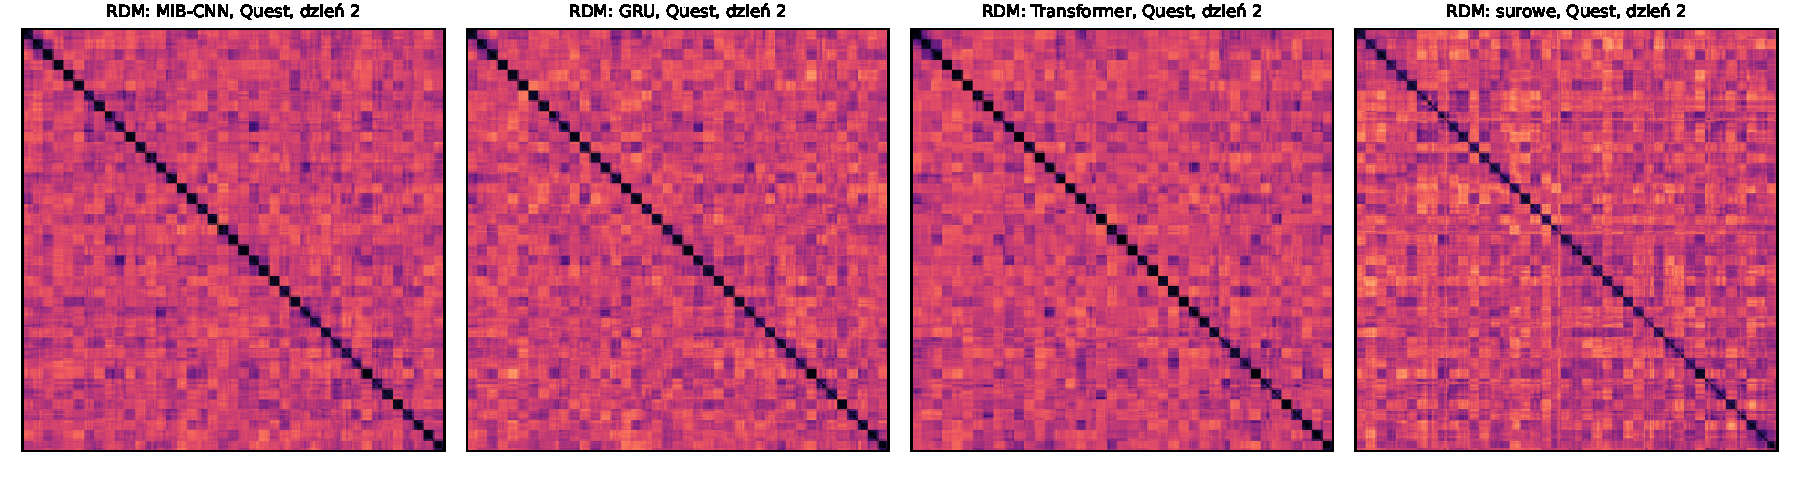
\includegraphics[width=0.95\linewidth]{rsa_rdm_examples.pdf}
\caption{Przykładowe RDM (Quest, \texttt{all}, próbki posortowane według uczestnika). Wyraźna struktura blokowo-diagonalna w modelach.}
\end{figure}

\section{Wnioski}
\begin{enumerate}
\item Ruch rzutu w VR jest silną cechą biometryczną, stabilną między dniami: najlepszy model (GRU, wszystkie cechy)
  osiąga Rank-1 = 90--96\% i EER = 1,1--3,9\% w protokole cross-day dla 41 osób.
\item \textbf{Ranking klasyfikatorów: GRU $>$ MIB-CNN $>$ Transformer.} GRU jest najdokładniejszy, najszybszy w treningu (ok. 13\,s)
  i daje najbardziej powtarzalne reprezentacje. MIB-CNN jest blisko i lepiej wykorzystuje rotacje.
  Transformer przy 410 sekwencjach treningowych bywa gorszy od baseline'u bez uczenia.
\item \textbf{Urządzenia:} najwięcej informacji biometrycznej dostarcza prawy (rzucający) kontroler,
  który sam prawie dorównuje kompletowi sensorów. Hełm niesie głównie informację statyczną (wzrost), a lewy kontroler najmniej.
  Spośród systemów najlepsze wyniki daje Vive (śr. 93,6\%), a najsłabsze Cosmos (87,4\%), dla którego dryf hełmu między dniami jest największy.
\item \textbf{Modalności:} pozycje są nieco bardziej informatywne niż rotacje, ale ich połączenie daje wyraźny zysk.
  RSA pokazuje, że kodują one różne aspekty tożsamości.
\item RSA wykazała, że o geometrii embeddingów decydują przede wszystkim dane wejściowe, a architektura ma wpływ wtórny.
  Dobór sensorów i cech jest więc ważniejszy niż dobór architektury.
\item Ograniczenia: zamknięty zbiór tożsamości (te same osoby w treningu i teście), brak walidacji hiperparametrów
  (stałe ustawienia dla wszystkich modeli), tylko 2 sesje na system. Główne źródło błędów to kilku uczestników,
  którzy zmienili sposób rzutu między dniami. Naturalnym rozszerzeniem jest uczenie metryczne (triplet / ArcFace)
  na otwartym zbiorze osób oraz scenariusze cross-device.
\end{enumerate}

\section*{Odtwarzalność}
Kod (\texttt{data.py}, \texttt{models.py}, \texttt{metrics.py}, \texttt{train.py}, \texttt{eda.py}, \texttt{analyze.py}, \texttt{rsa.py})
oraz instrukcja uruchomienia znajdują się w załączonym archiwum ZIP (\texttt{README.md}). Wszystkie liczby w raporcie
pochodzą z plików \texttt{results/*.json} i \texttt{results/*.csv} generowanych przez skrypty.
Kod napisano z pomocą narzędzia Claude, a wyniki zweryfikowano przez ponowne przeliczenie metryk z zapisanych embeddingów.

\end{document}
